\documentclass[reprint,
superscriptaddress,
 amsmath,amssymb,
 aps,
% prl,
prb,
%rmp,
%prstab,
%prstper,
%floatfix,
]{revtex4-1}


\usepackage{graphicx}% Include figure files
\usepackage{dcolumn}% Align table columns on decimal point
\usepackage{bm}
% \usepackage[all]{nowidow}
\usepackage{hyperref}
\hypersetup{colorlinks = true, linkcolor = [rgb]{0.19411,0.51882,0.667058}, urlcolor = [rgb]{0.125490,0.29542,0.1647058}, citecolor = [rgb]{0.75882,0.37411,0.14117}}


\widowpenalty10000
% \clubpenalty10000


\graphicspath{{../images/}}

\usepackage[toc,page]{appendix}

\newcommand{\nn}{\nonumber \\}
\newcommand{\bra}[1]{\langle{#1}|}
\newcommand{\ket}[1]{|{#1}\rangle}
\newcommand{\braket}[2]{\langle{#1}|{#2}\rangle}
%\def\comment#1{}
\def\comment#1{ [{\bf Comment:} {\sf #1}]}
\def\labell#1{\label{#1}}
%\def\labell#1{\label{#1}{\mbox{{\tiny #1}}}}
% \def\sectionp#1{{\par\em #1:--- }}
% \def\mostra#1{\refstepcounter{#1}\arabic{#1}}
\def\togli#1{}
\def\tr{\mbox{Tr}}
\def\iden{\openone}
\def\>{\rangle}
\def\<{\langle}


\usepackage{braket}

\def\>{\rangle}
\def\<{\langle}

% \def\section#1{{\par\em #1:--- }}
\usepackage[bottom]{footmisc}


\begin{document}
% \fbox{{\scriptsize Internal report \today}}

\title{Continuous variable }




\begin{abstract}

\end{abstract}

\date{\today}

\maketitle

% 









% \section{Dense coding}



\section{Teleportation}
Fig.~\ref{fig:tele}
\begin{widetext}
\begin{figure}[h!]
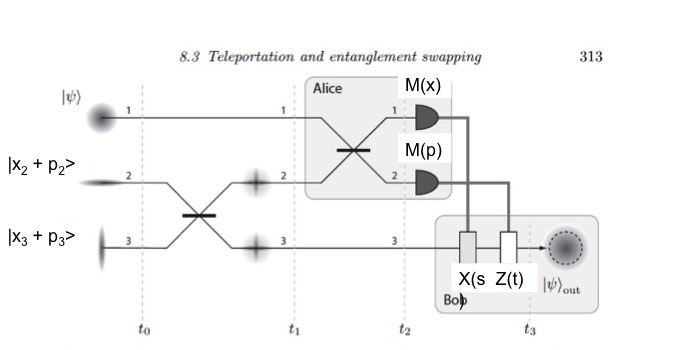
\includegraphics[trim = 0cm 0cm 0cm 0cm, clip, width=1.6\linewidth]{teleport.jpg}
\caption{\label{fig:tele}}
\end{figure} 


\end{widetext}


Protocol extended to CV by \cite{PhysRevA.49.1473,PhysRevLett.80.869}

\cite{kok2010introduction}
\begin{align}
\ket{p} = \int dx e^{i/\hbar p x} \ket{x}, \qquad 
\ket{x} = \int dx e^{i/\hbar x p} \ket{p}
\end{align}

Displacement operator


\begin{eqnarray}
X(s) &=& e^{-i/\hbar x \hat p}\\
X(s)\ket{x} &=&  \int dp e^{-i/\hbar p x} e^{-i/\hbar x \hat p} \ket{p} \\
   			&=& dp e^{-i/hbar p(x+s)} \ket{p} \\
   			&=&\ket{x+s}
\end{eqnarray}

This is the continuous-variable generalization of the Pauli X operator, in that it displaces the value of the state by amount $s$.


The analogue of the Pauli Z operator adds a state-dependent phase
% 
\begin{eqnarray}
Z(t ) &=& e^{i/\hbar t \hat x} \\
 e^{i/\hbar t \hat x} \ket{x} &=& e^{i/\hbar p x} \ket{x}
\end{eqnarray}

\noindent and acts on the momentum basis state $\ket{p}$ as
\begin{eqnarray}
Z(t)\ket{p}=\ket{p+t}.
\end{eqnarray}




Before the squeezing operator is applied, we set $t=0$.
\begin{enumerate}
\item At $t=t_0$, the vacuum states in mode 2 and 3 are squeezed. The quadrature operators become
\begin{align}
x_2(t_0) \rightarrow x_2(0) e^{r} \qquad p_2 \rightarrow p_2(0) e^{-r} \\
x_3(t_0) \rightarrow x_3(0) e^{r} \qquad p_3 \rightarrow p_3(0) e^{-r}
\end{align}
% 
\item The 50:50 beam splitter in modes 2 and 3 creates the approximate
Bell state necessary for teleportation, and this induces the quadrature
transformations
\begin{align}
x_2 (t_1) = \frac{x_2(t_0) + x_3(t_0)}{\sqrt 2} \qquad x_3 (t_1) = \frac{x_2(t_0) - x_3(t_0)}{\sqrt 2} \nonumber\\
p_2 (t_1) = \frac{p_2(t_0) + p_3(t_0)}{\sqrt 2} \qquad p_3 (t_1) = \frac{p_2(t_0) - p_3(t_0)}{\sqrt 2}
\end{align}
\item The second beam splitter induces the transformation
\begin{align}
x_1 (t_2) &= \frac{x_1(t_1) - x_2(t_1)}{\sqrt 2} \\
		  &= \frac{x_1(t_1)}{\sqrt 2} - \frac{x_2(t_0) + x_3(t_0)}{2} \label{b1}\\
% x_2 (t_2) &= \frac{x_1(t_1) - x_2(t_1)}{\sqrt 2} \nonumber\\
		  % &= \frac{x_1 (t_0)}{\sqrt 2} +  \frac{x_2(t_0) + x_3(t_0)}{ 2} label{b1} \\
% p_1 (t_2) &= \frac{p_1 (t_1) + p_2(t_1)}{\sqrt 2} \nonumber \\
p_2 (t_2) &= \frac{p_1(t_1) + p_2(t_1)}{\sqrt 2} \\
		  &=\frac{p_1 (t_0)}{\sqrt 2} +  \frac{p_2(t_0) + p_3(t_0)}{ 2} 
\end{align}
% 

\noindent Now, if we rearrange Eq.~\eqref{b1} to make $x_2(t_0)$ the subject, and identify that $x_1(t_1) = x_1 (t_0)$
\begin{align}
x_2(t_0) &= -2 x_1(t_2)+ \sqrt 2x_1(t_1) - x_3(t_0) \\
		% &= -2 x_1(t_2)+ \sqrt 2x_1(t_0) - x_3(0) e^{-r} \\
p_2(t_0) &= -  2p_2(t_2)  + \sqrt 2 p_1 (t_0) - p_3 (t_0)
\end{align}

\color{blue}
 Now, for Bob, $x_3(t_2) = x_3 (t_1),p_3(t_2) = p_3 (t_1)$, whose state is now
\begin{align}
 x_3 (t_2) &= \frac{-2 x_1(t_2)+ \sqrt 2x_1(t_1) - x_3(t_0) - x_3(t_0)}{\sqrt 2} \nonumber\\
		   &= -\sqrt 2 x_1(t_2 ) + x_1(t_0) - \sqrt 2 x_3(0)e^{-r} \\
 % \frac{2 x_2(t_2)- \sqrt 2x_1(t_0) - x_3(t_0) - x_3(t_0)}{\sqrt2}\\
p_3 (t_2) &=   \frac{p_2(t_0) - p_3(t_0)}{\sqrt 2} \\
		  &=   \frac{-  2p_2(t_2)  + \sqrt 2 p_1 (t_0) - p_3 (t_0) - p_3(t_0)}{\sqrt 2} \\
		  &=  p_1(t_0)- \sqrt2p_2(t_2) - \sqrt2 p_3 (t_0)
\end{align}

\item Alice measures the position quadrature $x_1(t_2)$ in mode 1, yielding
the outcome $s/\sqrt2$, and she measures the momentum quadrature
$p_2(t_2)$ in mode 2, yielding the outcome $t/\sqrt2$. She sends these measurement outcomes to Bob.
\noindent applies the displacements
\begin{align}
X(u) = \exp(-2 i s \hat p_3) \qquad Z(t) = \exp(2i t \hat x_3)
\end{align}
The output quadratures at Bob's mode become
\begin{align}
x_3 = x_1 -\frac{\sqrt2 x_3}{e^r} \qquad p_3 = p_1 - \frac{\sqrt2 p_3}{e^r}
\end{align}
\end{enumerate}

Here the input quadratures are teleported to the output quadratures up to a factor $\frac{\sqrt2 p_3}{e^r}$. In the limit of infinite squeezing $\rightarrow \infty$, the teleportated state is perfect.



\section{Entanglement swapping}

\section{Entanglement distillation}

Entanglement distribution between distant parties is an essential component to most quantum communication protocols \cite{PhysRevLett.81.5932}. As it has been discussed, entanglement is a resource in a quantum network, and it is of interest for distant parties to share maximally entangled states. 

In practice the transmission channel is never perfect, and noise due to interaction with the environment or imperfect gate operations will reduce the entanglement of a state. If one has several copies of some less than maximally entangled state available, it is possible for two parties to concentrate or distill the entanglement.

In contrast to the qubit version, however, it has been proven that for Gaussian states
it is impossible to distill more entanglement by using Gaussian operations \cite{PhysRevLett.89.137904,PhysRevLett.89.137903,PhysRevA.66.032316}. In order to to distill from Gaussian input states, non-Gaussian operations are necessary.
 
Proposal \cite{eisert2004distillation}, one variant experimentally realized by photon-subtraction \cite{takahashi2010entanglement}.

\section{Quantum computing}



\subsection{Quantum gates}

Gates for the qubit circuit model and the analogous operations for CV are summarised in Table~\ref{tabgates}. \cite{RevModPhys.84.621}
\begin{table}
\begin{tabular}{ |c|c| } 
 \hline
 Circuit model &  CV cluster state \\ 
  \hline\hline
 Pauli $X$ & $X(s) = \exp[-i s \hat p]$  \\ 
 Pauli $Z$ & $Z(t) = \exp[i t \hat q]$  \\ 
 Phase gate & $\hat P (\eta) = \exp[i \eta \hat x^2]$ \\
Hadamard   & $F=\exp[i \frac{\pi}{8}(\hat p^2+\hat q^2)]$ \\
$C_Z$	   & $C_Z= \exp[\frac{i}{2}q_1 \otimes q_2]$ \\
CNOT 	   & $C_X = \exp[-2i\hat x_1 \otimes \hat p_2]$\\
\hline
\end{tabular}
\caption{\label{tabgates}}
\end{table}
%  

The operators $X,Z$ can be interpreted as displacement operators
\begin{align}
D(\alpha) = \exp(\alpha \hat a^\dagger - \alpha^* \hat a)
\end{align}
which correspond to a translation in phase space. $X$ is a translation in position, and Z is a displacement in momentum.

The X and Z operators can be written as 
X = D(s/2), Z = D(it/2)



The Fourier gate F is the Gaussian analogue of the qubit Hadamard gate, which corresponds to a $\pi/2$ rotation in phase space, and transforms the quadrature eigenstates from one to another:

\begin{eqnarray}
F = \exp(i\pi/4)\exp(\frac{i\pi}{4} \hat a^\dagger \hat a) = (\hat p^2+\hat x^2)
\end{eqnarray}

\begin{eqnarray}
F\ket{s}_x = \ket{s}_p
\end{eqnarray}


The controlled-phase gate, $C_Z$ is a two-mode Gaussian gate. It is defined as

\begin{eqnarray}
E_z = \exp\left(\frac{i}{2} \hat x_1 \otimes \hat x_2 \right).
\end{eqnarray}

It transforms on the quadrature eigenstates as
\begin{eqnarray}
C_Z \ket{s}_1 \ket{t}_2 = \exp(i s_1 t_2)/2 \ket{s}_1\ket{t}_2  
\end{eqnarray}


It transforms the momentum quadratures according to

\begin{eqnarray}
\hat p_1 \rightarrow \hat p_1 + \hat x_2, \qquad \hat p_2 \rightarrow \hat p_2 + \hat x_1
\end{eqnarray}

\subsection{Cluster state/ measurement based}



\cite{PhysRevLett.97.110501}
The advantage of this approach is that both the cluster state preparation and comutation can be performed deterministically.

Once the state has been created, a sequence of one-mode (separable) measurement 


The one-qubit teleportation give insight into how the cluster-state evolves in this model


\begin{figure}
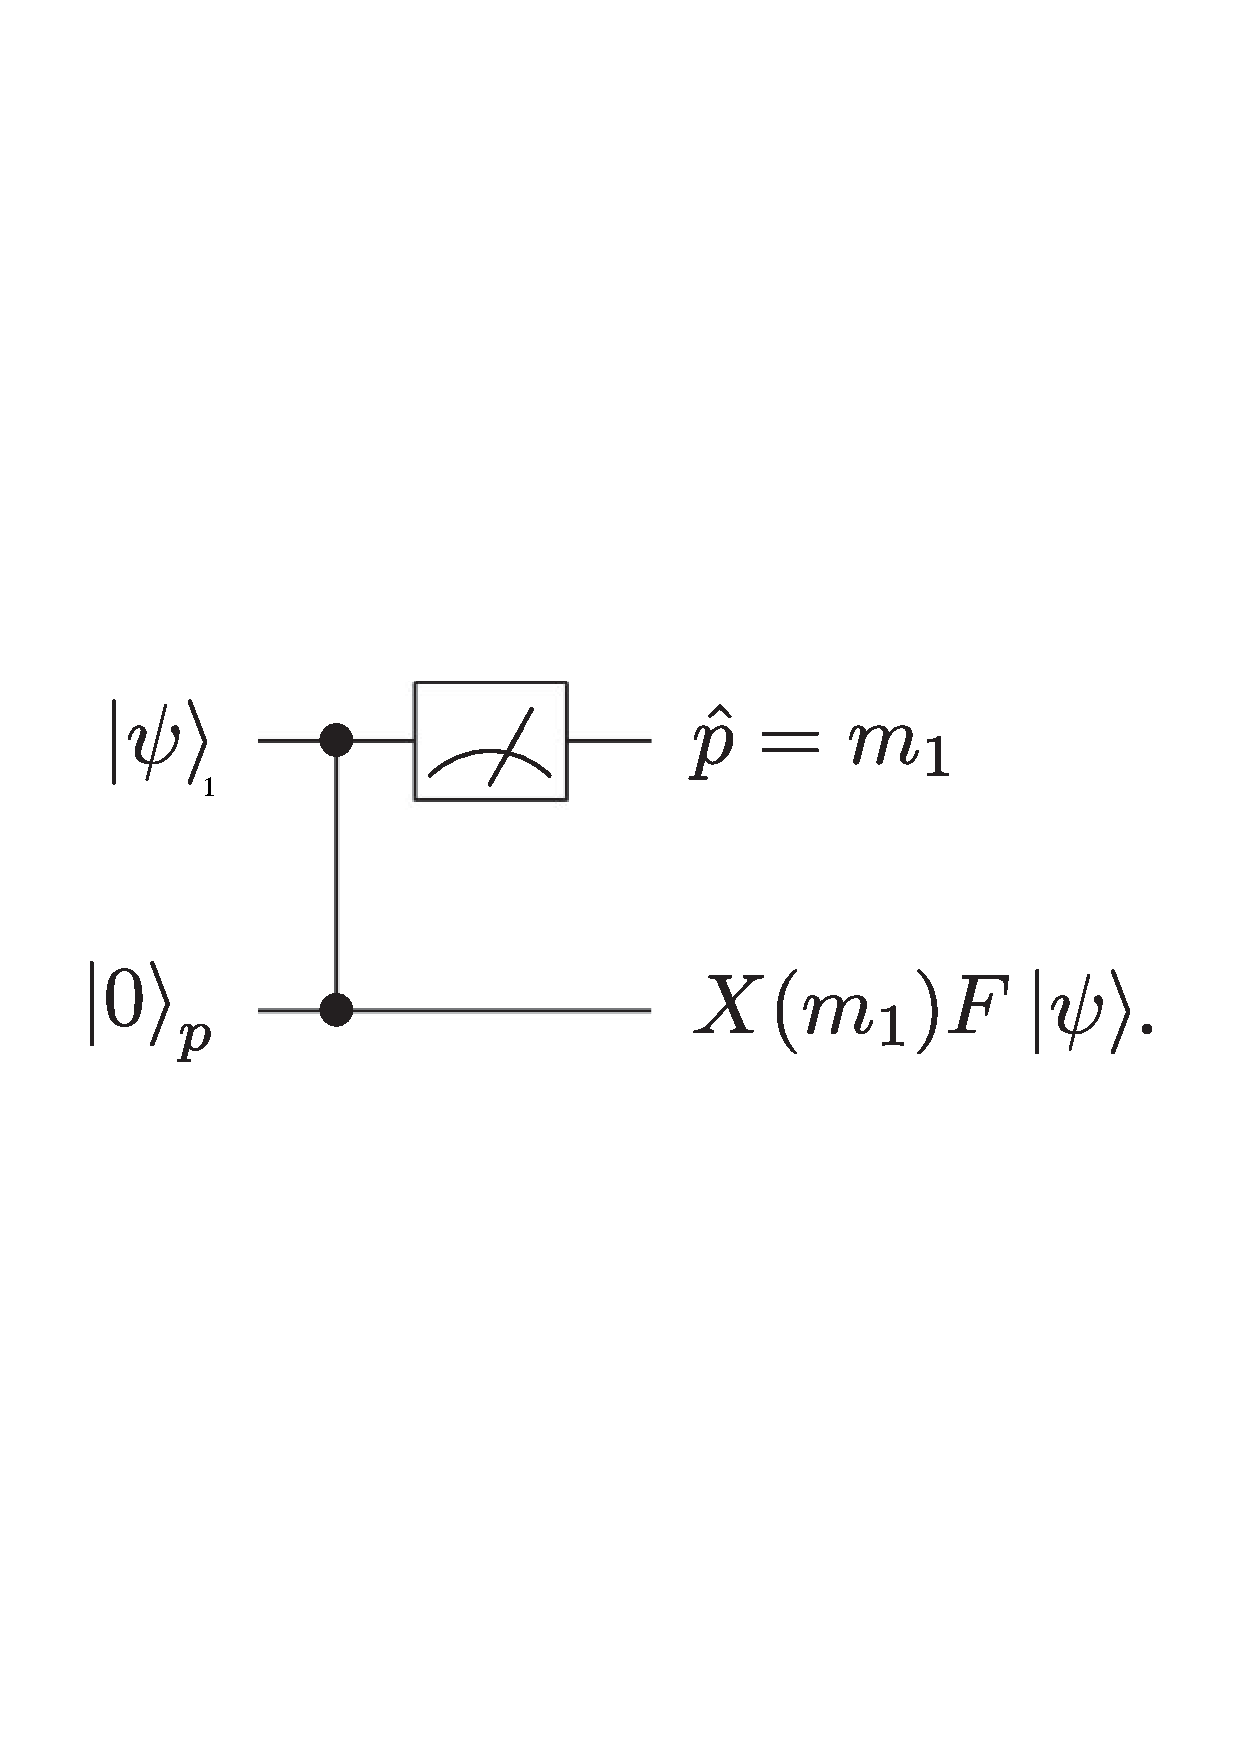
\includegraphics[trim = 0cm 10cm 0cm 10cm, clip, width=0.75\linewidth]{one_qubit_teleport.pdf}
\caption{\label{fig:cluster_Teleport}}
\end{figure}

 Consider perfect squeezing, where the second mode is a momentum eigenstate $\ket{0}_p$. Initially, the state is 


\begin{eqnarray}
\ket{\psi}\ket{0}_p = \frac{1}{\sqrt {2\pi}} \int dx_1 dx_2 \psi(x_1)\ket{x_1}\ket{x_2}
\end{eqnarray} 

Applying the $C_Z$ gate results in


\begin{eqnarray}
\frac{1}{2\pi} \int dx_1 dx_2 \psi(x_1) \exp(i x_1 x_2/2)\ket{x_1}\ket{x_2}
\end{eqnarray}

After measuring $\hat p_1$, the state is projected onto $\ket{m_1}\bra{m_1}$, we have

$\braket{m_1|q_1}= 1/2\pi \exp(-iq_1 m_1/2)$


\begin{eqnarray}
\frac{1}{4\pi}\int d x_1 d x_2 \psi(x_1) \exp(i x_1 (q_2 - m_1)) q_2
 \end{eqnarray}
 
Applying the correction $X(m_1)$ gives back the initial state $\ket{\psi}$

% \begin{enumerate}
% 	\item
% 	\item mode 1 and 2 are entangled using a $C_Z$  gate
% 	\item Measurement in $\hat p$ is performed on mode 1, resulting in outcome $m_1$
% \end{enumerate}

We can now consider the teleportation of a quantum gate, which is the key of the measurement-based quantum computing.
Consider a variation of the above circuit, where the only difference is the addition of a unitary that is diagonal 
in the computational basis, and therefore commutes with the CPHASE gate, for example $U=\exp(i f(\hat x))$. 


\begin{figure}[thb]
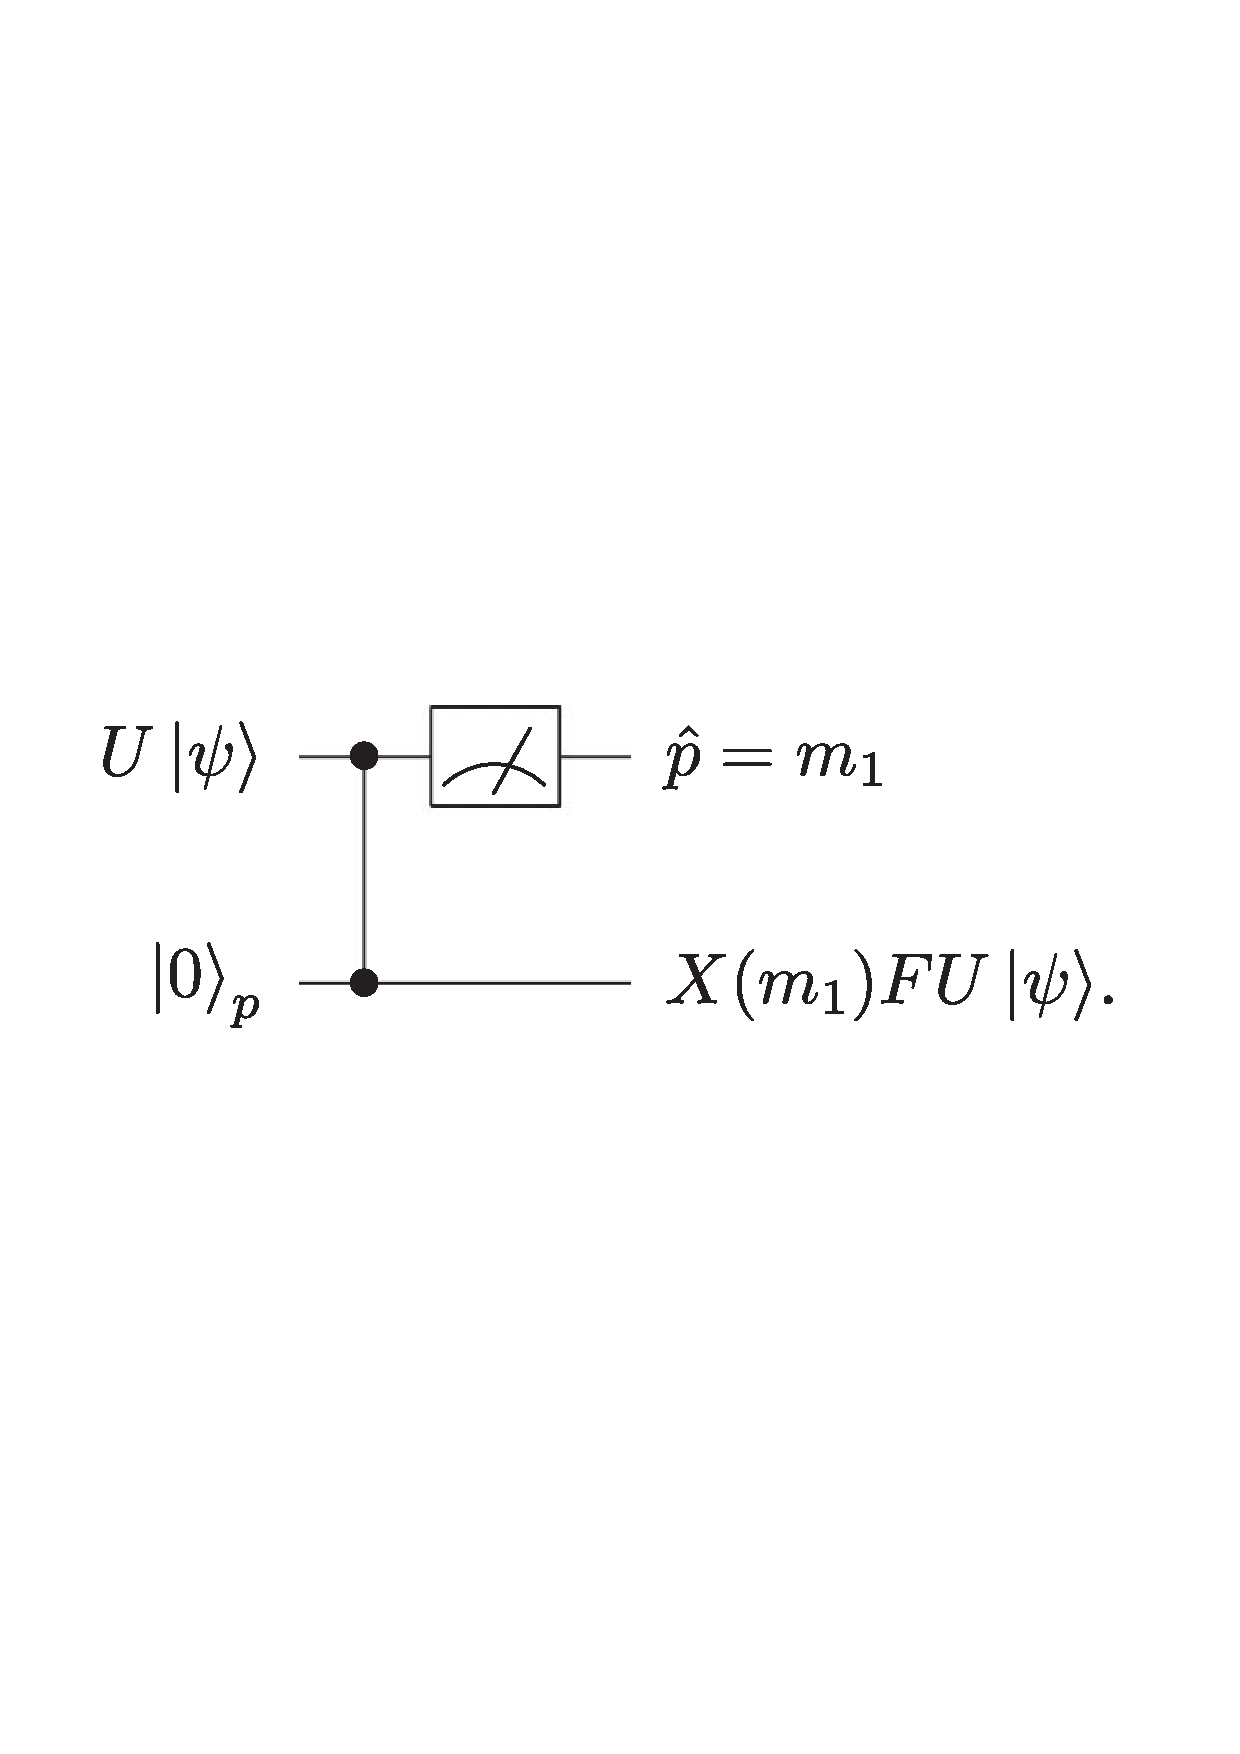
\includegraphics[trim = 0cm 10cm 0cm 10cm, clip, width=0.8\linewidth]{teleport_circ2.pdf}
\\
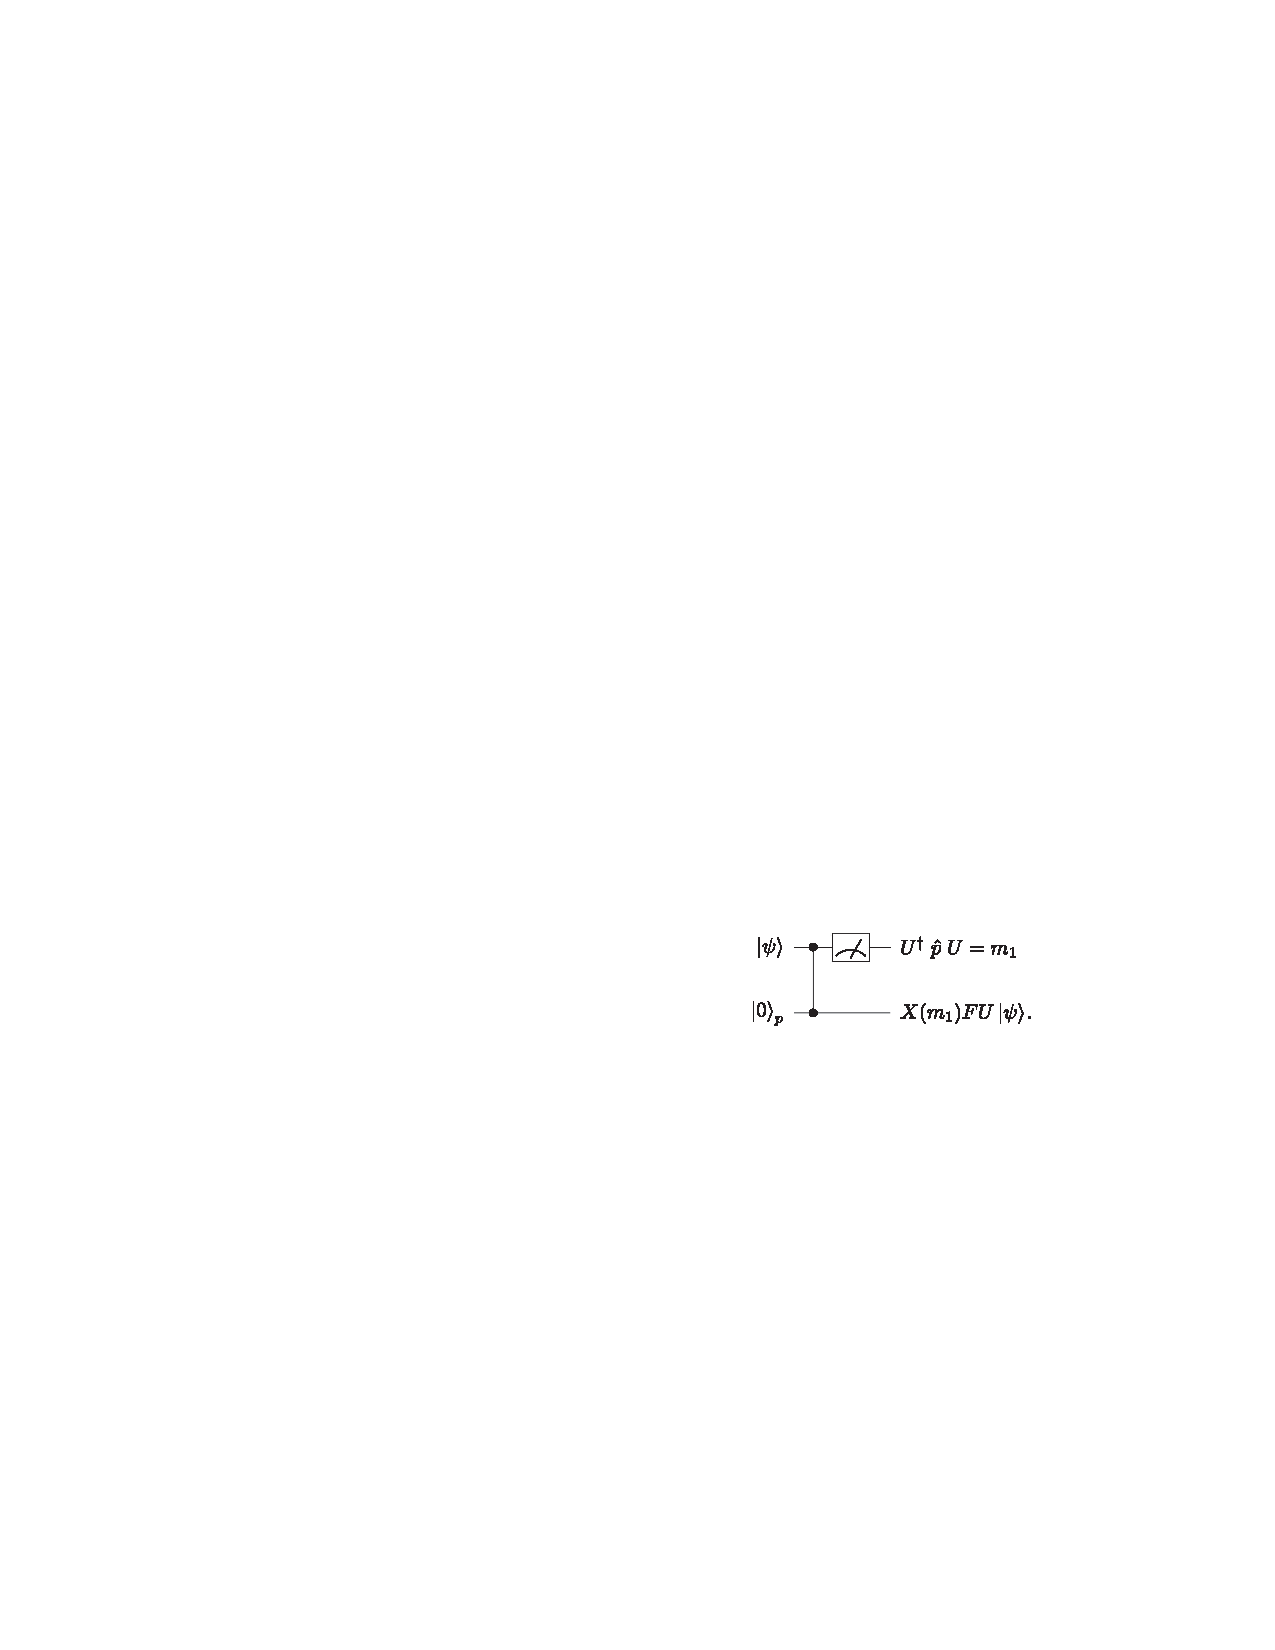
\includegraphics[trim = 0cm 0cm 0cm 0cm, clip, width=0.8\linewidth]{teleport_circ3.pdf}
\caption{\label{fig:cluster_Teleport23}}
\end{figure}




We have just shown that 
by performing a measurement in the basis $U\hat x U^\dagger$, we can absorb the gate into the measurement. 

% \section{}
\begin{itemize}
	\item addition of any non-gaussian projective measurement allows universal QC using CV cluster states
	\item multimode Gaussian operations can be made in any order
\end{itemize}


\bibliography{reference}


\begin{eqnarray}
\end{eqnarray}

\end{document}

\begin{align}
\end{align}